% !TEX root = main.tex
\chapter[head={\CP violation in the $B$-meson sector},tocentry={$\symbfsf{C{}P}$ violation in the $\symbfsf{B}$-meson sector}]
{$\symbfsf{C{}P}$ violation in the $\symbfsf{B}$-meson sector}
\label{chap:CPV}

Due to the high mass of the \bquark-quark it offers a large variety of decays in which the elements of the $CKM$ marix can be analysed.
It is therefore a perfect candidate to study effects of \CP violation and as a consequence thereof the complex phase of the matrix. This
chapter describes first the process of neutral meson mixing by the example of uncharged \B-mesons before explaining the
three classes of \CP violation. Finally the underlying formalism when measuring \CP violation time dependently is presented.

\section[head={$B$-meson mixing},tocentry={$B$-meson mixing}]{$\symbfsf{B}$-meson mixing}
\label{sec:Bmixing}

As explained in \cref{sec:unitarityTriangle} the mass eigenstates and the eigenstates to the weak interaction are not identical for
quarks. The same holds for bound states of quarks like \B-mesons. Studying the system of a \Bz (\bquarkbar\dquark) and a \Bzb-meson
(\bquark\dquarkbar), the most general description to deduce the time evolution is the Schrödinger equation:
\begin{equation}
i\frac{d}{dt}\begin{pmatrix} \Bz \\ \Bzb \end{pmatrix} = H \begin{pmatrix} \Bz \\ \Bzb \end{pmatrix},
\end{equation}
where $M$ and $H$ are hermitian matrices with $m_{11}=m_{22}$ and $\Gamma_{11}=\Gamma_{22}$ due to the $CPT$ theorem. Diagonalising
the matrix leads to the eigenvales $\mu_{1,2}=m_{1,2}-\frac{i}{2}\Gamma_{1,2}$ with the masses $m_{1,2}$ and decay widths
$\Gamma_{1,2}$  of the mass eigenstates. In the \Bz-meson system the mass eigenstates are denoted as $\B_L$ and $\B_H$ and
analogous both the masses with $m_L$ and $m_H$ and the decay widths with $\Gamma_L$ and $\Gamma_H$. The mass eigenstates
can be expressed as
\begin{equation}
\begin{split}
\left|B_H\right>&\sim p\left|\Bz\right>-q\left|\Bzb\right>\\
\left|B_L\right>&\sim p\left|\Bz\right>+q\left|\Bzb\right>
\end{split}
\end{equation}
where $p$ and $q$ are constrained to fulfil $\left|p\right|^2+\left|q\right|^2=1$. Further the quantities
\begin{align}
\dm&=m_H-m_L\\
\DG&=\Gamma_L-\Gamma_H
\end{align}
can be defined. For the time evolution of the flavour eigenstates holds
\begin{equation}
\begin{split}
\left|\Bz\!\left(t\right)\right>&=\left|\Bz\right>g_+-\frac{q}{p}\left|\Bzb\right>g_-\\
\left|\Bzb\!\left(t\right)\right>&=\left|\Bzb\right>g_--\frac{p}{q}\left|\Bz\right>g_+
\end{split}
\end{equation}
with $g_\pm=\frac{1}{2}\left(e^{-i\mu_Ht}\pm e^{-i\mu_Lt}\right)$. Using this the probability that an initially produced
\Bz meson oscillates after a given time $t$ is
\begin{equation}
\left|\left<\Bz\Big|\Bzb\!\left(t\right)\right>\right|^2=\frac{1}{4}\left|\frac{q}{p}\right|^2
\left(e^{-\Gamma_Ht}+e^{-\Gamma_Lt}-2e^{\frac{1}{2}\left(\Gamma_H+\Gamma_L\right)t}\cos\left(\dm t\right)\right)
\end{equation}
Analogous the probablity for an initially produced \Bzb and the unmixed cases can be calculated. One sees, that the probability
always oscillates with with the frequency \dm. The corresponding Feynmangraphs are shown in \cref{fig:FeynmanMixing}.

\begin{figure}[tbp]
	\centering
	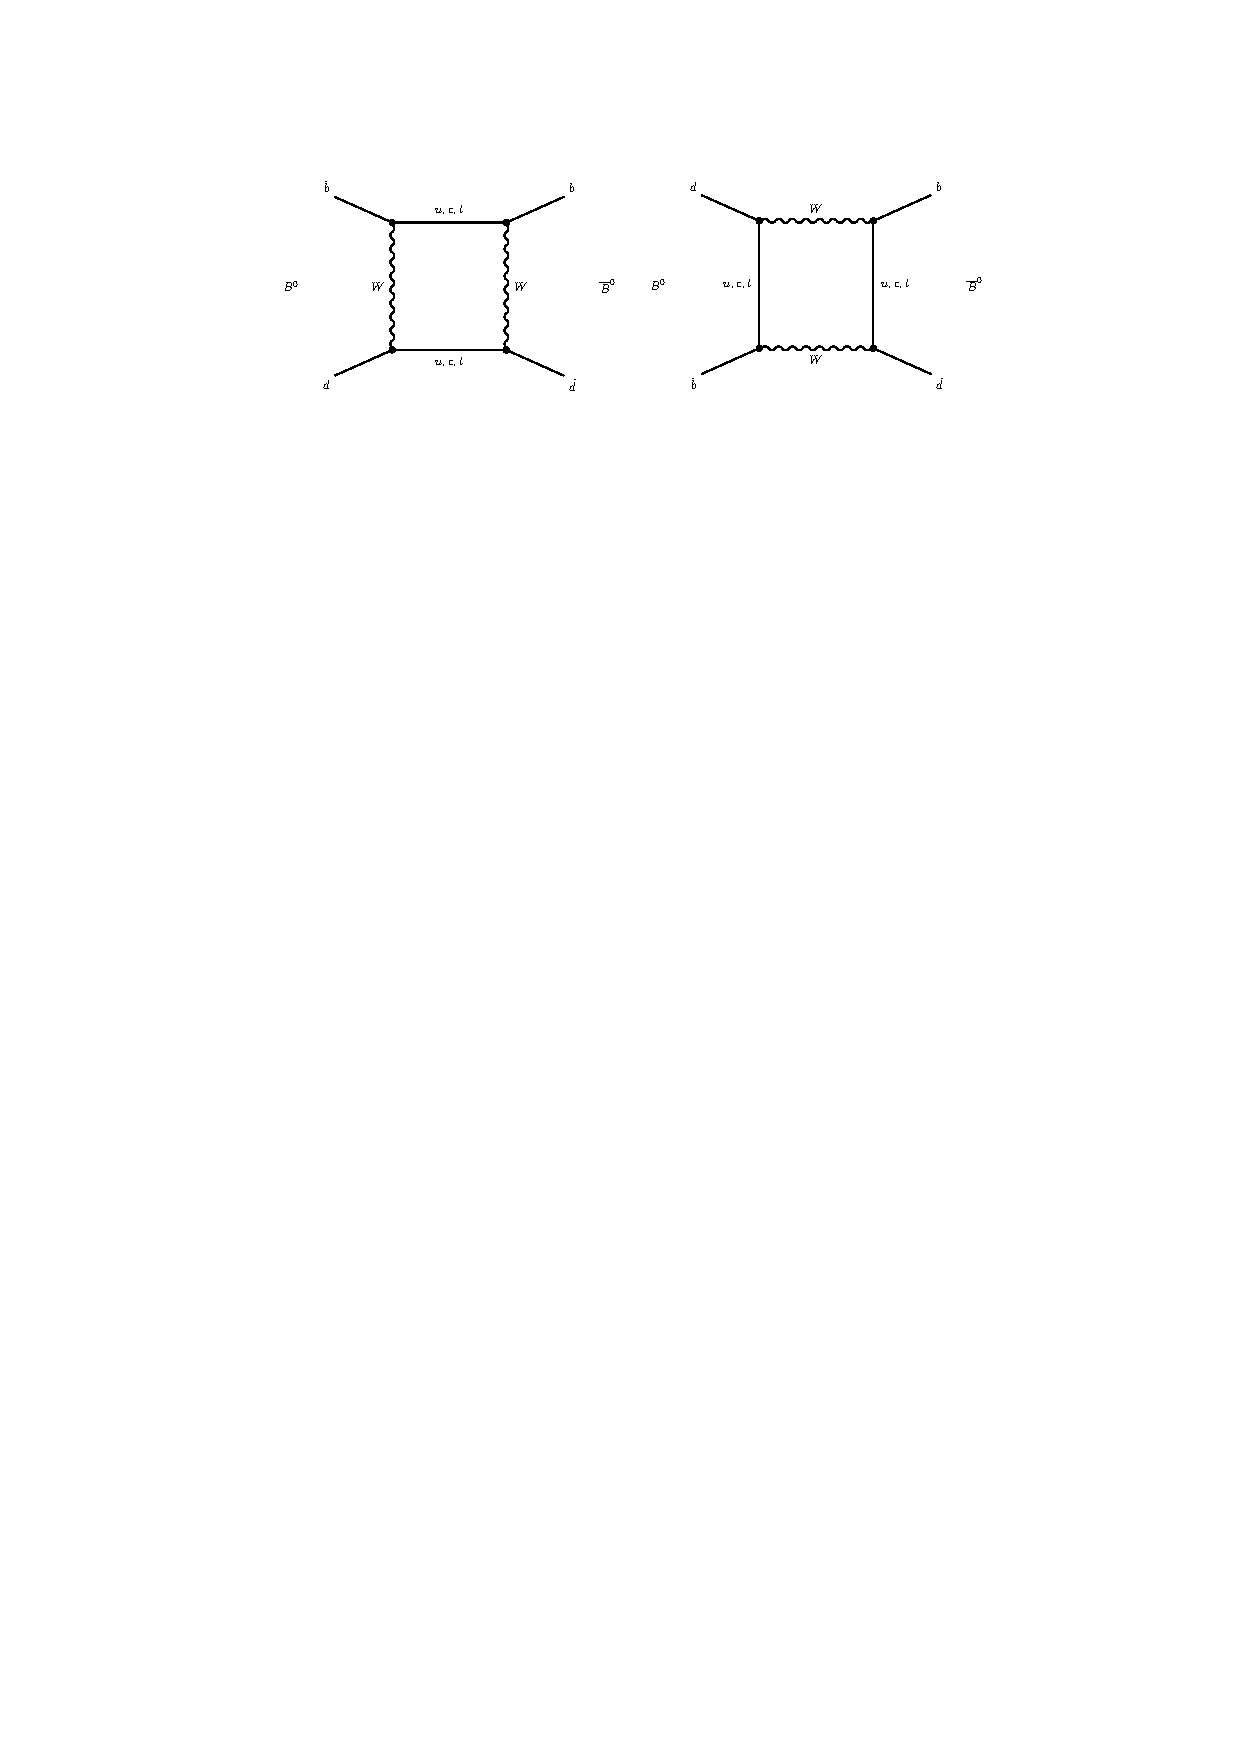
\includegraphics[width=0.9\textwidth]{03CPV/figs/FeynmanMixing.pdf}
	\caption{box diagrams of lowest order for the \Bz-\Bzb-oscillation. Both diagrams are dominated by the \tquark-quark.}
	\label{fig:FeynmanMixing}
\end{figure}

\section[head={Types of \CP violation},tocentry={Classes of \CP violation}]{Classes of $\symbfsf{C{}P}$ violation}
\label{sec:CPVClasses}

As described in \cref{sec:symmetriesInSM} the the \CP symmetry is broken by the weak interaction. To further understand
the different types of \CP violation first the following decay amplitudes are introduced:
\begin{equation}
\begin{split}
\Af = \left<\,f\,\Big|T\Big|\Bz\right>\hspace{1cm}\Afbar = \left<\,\fbar\,\Big|T\Big|\Bz\right>\\
\Abarf = \left<\,f\,\Big|T\Big|\Bzb\right>\hspace{1cm}\Abarfbar = \left<\,\fbar\,\Big|T\Big|\Bzb\right>
\end{split}
\end{equation}
Here $T$ denotes the transition matrix from the \B-meson in some final state \f or \fbar. Together with the
mixing parameters $p$ and $q$ the helpful quantities $\lambda_f$ and $\lambda_{\fbar}$ can be introduced:
\begin{equation}
\Lf=\frac{q}{p}\frac{\Abarf}{\Af}\hspace{0.5cm}\text{and}
\hspace{0.5cm}\Lfbar=\frac{p}{q}\frac{\Afbar}{\Abarfbar}
\end{equation}
Now the three types of \CP violation can be separated.

\subsection[head={Direct \CP violation},tocentry={Direct \CP violation}]{Direct $\symbfsf{C{}P}$ violation}
\label{sec:DirectCPV}

Direct \CP violation or \CP violation in decay means that a specific decay amplitude differs between the particle and  its
corresponding antiparticle. So the conditions $\left|\Af\right|\neq\left|\Abarfbar\right|$ and
$\left|\Afbar\right|\neq\left|\Abarf\right|$ hold and following this also $\left|\Lf\right|\neq1$ and $\left|\Lfbar\right|\neq1$.
For \B-mesons this has been measured in the decay mode $\Bp\to\kaon\pion$

\subsection[head={Mixing \CP violation},tocentry={Mixing \CP violation}]{Mixing $\symbfsf{C{}P}$ violation}
\label{sec:MixingCPV}

Indirekt \CP violation (\CP violation during mixing) means that the transition probability from a \Bz-meson to a \Bzb meson
and the other way round are different. As the name implies this type of \CP violation can only occur for neutral particles
which can oscillate in their antiparticle. In terms of the introduced quantities in \cref{sec:CPVClasses} this means that
$\left|\frac{q}{p}\right|\neq1$ and therefore also $\left|\Lf\right|\neq1$ and $\left|\Lfbar\right|\neq1$.

\subsection[head={Interference \CP violation},tocentry={Interference \CP violation}]{Interference $\symbfsf{C{}P}$ violation}
\label{sec:InterferenceCPV}

The third type of \CP violation occurs in the interference of direct decay and decay after mixing.

\section[head={Time dependent measurement of \CP violation},tocentry={Time dependent measurement of \CP violation}]
{Time dependent measurement of $\symbfsf{C{}P}$ violation}
\label{sec:TimeDependentCPV}

